        %%******************************************%%
        %%                                          %%
        %%        Modello di tesi di laurea         %%
        %%            di Andrea Giraldin            %%
        %%                                          %%
        %%             2 novembre 2012              %%
        %%                                          %%
        %%******************************************%%

\begin{document}
    \frontmatter
    \begin{titlepage}
    \begin{center}
        \begin{LARGE}
            \textbf{\myUni}\\
        \end{LARGE}

        \vspace{10pt}

        \begin{Large}
            \textsc{\myDepartment}\\
        \end{Large}

        \vspace{10pt}

        \begin{large}
            \textsc{\myFaculty}\\
        \end{large}

        \vspace{30pt}
        \begin{figure}[htbp]
            \centering
            
\includegraphics[height=5cm]{unipd-logo.png}
        \end{figure}
        \vspace{30pt}

        \begin{LARGE}
            \textbf{\myTitle}\\
        \end{LARGE}

        \vspace{10pt}

        \begin{large}
            \textsl{\myDegree}\\
        \end{large}

        \vspace{40pt}

        \begin{large}
            \begin{flushleft}
                \textit{Supervisor}\\
                \vspace{5pt}
                \profTitle\ \myProf
            \end{flushleft}

            % You can tweak the spacing to have professor and student names on the same line
            % useful if the page is broken by a long thesis title and you need more space
            \vspace{-52pt}

            \begin{flushright}
                \textit{Candidate}\\
                \vspace{5pt}
                \myName \\
                \vspace{5pt}
                \textit{ID} \myID
            \end{flushright}
        \end{large}

        \vspace{40pt}

        \line(1, 0){338} \\
        \begin{normalsize}
            \textsc{Academic Year \myAA}
        \end{normalsize}
    \end{center}
\end{titlepage}

    \clearpage
\phantomsection
\thispagestyle{empty}

\hfill
\vfill

\noindent\myName: \textit{\myTitle,}
\myDegree,
\textcopyright\ \myTime.

    \cleardoublepage
\phantomsection
\pdfbookmark{Summary}{summary}
\begingroup
\let\clearpage\relax
\let\cleardoublepage\relax
\let\cleardoublepage\relax

\chapter*{Summary}

This document describes the work done during the 750-hours final project at \href{https://www.221e.com/about-us}{221e S.r.l.}\\
The project's goal is to architect and develop a cloud-based system capable of ingesting and processing data from heterogeneous IoT sensors so that a knowledge database can be built.\\
The system must be designed to be scalable and fault-tolerant, and it must be platform-agnostic.\\
This document is going to describe the company, the idea behind the project, the work done and an assessment of what I developed and learned during my internship.\\

%\vfill

%\selectlanguage{english}
%\pdfbookmark{Abstract}{Abstract}
%\chapter*{Abstract}

%\selectlanguage{italian}

\endgroup

\vfill

    \cleardoublepage
\phantomsection
\pdfbookmark{Acknowledgements}{acknowledgements}

\begin{flushright}{
    \slshape
    ``Te ghe da pomparghe drio''} \\
    \medskip
    --- Federico Gallo
\end{flushright}


\bigskip

\begingroup
\let\clearpage\relax
\let\cleardoublepage\relax
\let\cleardoublepage\relax

\chapter*{Acknowledgements}

\noindent \textit{Prof. \myProf, my thesis supervisor, deserves my deepest gratitude for his exceptional support and guidance throughout the completion of this research.}\\
\noindent \textit{My family, for their encouragement and understanding throughout this academic endeavour, has my heartfelt thanks.}\\
\noindent \textit{I am truly grateful to Luca Perosa, Bledar Gogaj, Marco Lionello, and all my peers at SCAI ITEC, for their unwavering support when I made the decision to pursue a Master’s degree.}\\
\noindent \textit{I extend my sincere appreciation to PhD. Roberto Bortoletto, my company tutor, and all my colleagues in 221e for their invaluable support and guidance throughout my final project.}\\
\noindent \textit{Last but not least, I want to give a shoutout to all my friends for having my back and just being there through high and lows. Your friendship means a lot to me, and I appreciate the support and good times we've shared.}\\
\bigskip

\noindent\textit{\myLocation, \myTime}
\hfill \myName

\endgroup

    \cleardoublepage
\pdfbookmark{\contentsname}{tableofcontents}
\setcounter{tocdepth}{2}
\tableofcontents
%\markboth{\contentsname}{\contentsname}
\clearpage

\begingroup
    \let\clearpage\relax
    \let\cleardoublepage\relax
    \let\cleardoublepage\relax

    % Figures list
    \phantomsection
    \pdfbookmark{\listfigurename}{lof}
    \listoffigures

    \vspace*{8ex}

    % Tables list
    \phantomsection
    \pdfbookmark{\listtablename}{lot}
    \listoftables

    \vspace*{8ex}
\endgroup

\cleardoublepage

    \cleardoublepage

    \mainmatter
    \chapter{Introduction}
\label{cap:introduction}

\section{The Company}
\href{https://www.221e.com/about-us}{221e S.r.l.}\footcite{site:221e}, an innovative startup established in 2012 in Italy, has business units in Padova, Treviso, and Bergamo. The company leverages advancements in IT, microelectronics, sensors, and control algorithms to develop miniaturized wireless embedded systems.

Operating under a dual-layer business model, 221e offers:
\begin{enumerate}
    \item OEM (Original Equipment Manufacturer) services to third-party clients needing a technology partner for product development. This involves R\&D contracts followed by commercial agreements for the supply of engineered systems or technology licensing.
    \item Finished products, particularly general-purpose multi-sensor hardware platforms, to direct customers or distributors.
\end{enumerate}

Targeting the Wearable Devices market and the broader Internet of Things (IoT) industry, 221e capitalizes on the limitless applications within these fields. The name 221e, which represents the infinity Unicode character (\(\infty\)), reflects this boundless potential.

Despite being a small business, 221e is rapidly growing, driven by innovation and entrepreneurship, riding the wave of IoT and wearable device advancements.

\begin{figure}[htbp]
    \centering
    
\includegraphics[height=2cm]{221e_logo.png}
    \caption{221e's logo}
\end{figure}

\begin{figure}[htbp]
    \centering
    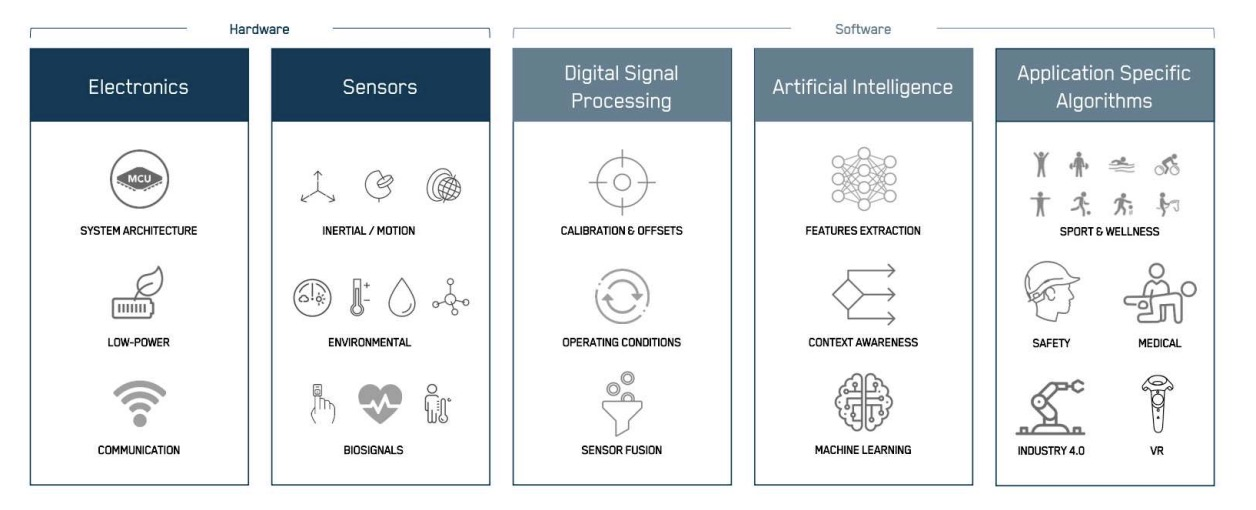
\includegraphics[width=\textwidth]{221e_applications.png}
    \caption{221e's technology echosystem}
\end{figure}


\newpage
\section{Idea}

The idea behind the project is to create a cloud-agnostic architecture for the 221e's IoT devices. The architecture should be able to ingest data from multiple sources, store it and  analyze it. The architecture should be able to scale horizontally and vertically, and should be able to be deployed on multiple cloud providers.


%<\section{Thesis outline}

%\begin{description}
 %   \item[{\hyperref[cap:requirements]{The second chapter}}] describes the high level requirements.
  %  \item [{\hyperref[cap:technologies]{The third chapter}}] describes the technologies taken into consideration for the project.
   % \item[{\hyperref[cap:method]{The fourth chapter}}] describes how the solution has been implemented.
    %\item[{\hyperref[cap:results]{The fifth chapter}}] assess the results of the project.
    %\item[{\hyperref[cap:conclusion]{The last chapter}}] describes the conclusion of the project and the future work.
%\end{description}

    \chapter{Objectives and requirements}
\label{cap:requirements}
\intro{In this chapter are discussed the main objectives and requirements of the architecture to be developed.}\\

\section{Cloud Infrastructure}
The system must be able to ingest, store and process large amount of IoT data leveraging the power of any cloud provider present in the market. The final product to be developed is a cloud agnostic architecture that can be deployed on any cloud provider. The main advantage of a cloud agnostic architecture is that it can be deployed on any cloud provider, virtually without any modification. This allows customers to choose the cloud provider that best fits his needs.
The providers taken into account to develop the architecture during this project are the following: \href{https://www.arubacloud.com/}{Aruba Cloud}\footcite{site:aruba-cloud}, \href{https://aws.amazon.com/it/}{Amazon Web Services}\footcite{site:aws} and \href{https://azure.microsoft.com/it-it/}{Microsoft Azure}\footcite{site:azure}. 
AWS and Azure were chosen because the already developed experience by the company and me while Aruba Cloud was chosen because of a partnership between the company and the cloud provider that started during the development of the project.\\


\section{Data collection}
The system must be able to ingest data from online devices and on-premise data sources. 
Online devices are devices that are connected to the internet and can send data to the cloud via MQTT protocol.
On-premise data source are offline files that are stored on a local machine and must be uploaded to the cloud. The system must provide a way to upload these files to the cloud.
\section{Data processing}
The system must be able to preprocess the data before storage. The preprocessing of the data includes data validation, data cleaning and data transformation, this can be done in cloud or on-premise. The system must be also able to process data after storage. The processing of the data includes data analysis and machine learning operations. The goal of the data processing is to extract useful information from the data and to provide insights to the customer.\\ 

\section{Security}
Security is a major concern for the system. In certain scenarios, the data collected could be sensitive and thus must be protected both in transit and at rest.
    \subsection{Security in transit}
    Data in transit are transfered using MQTT protocol which is not encrypted by default. The system must provide a way to encrypt and secure the data in transit. MQTT brokers however supports authentication and authorization through certificates as well as TLS/SSL encryption. Using a broker that supports these features is a must.
    
    \subsection{Security at rest}
    Data at rest is stored in cloud storage. The cloud storage must provide a way to encrypt the data at rest. The system must also provide a way to manage the encryption keys. Each cloud service provider taken into account provide a way to encrypt data at rest and manage the encryption keys.\\ 
    Furthermore, each cloud provider uses a shared responsibility model for security.
    
    \newpage
    \subsubsection{Aruba Shared Responsibility Model}
    \href{https://kb.arubacloud.com/en/computing/use-and-technology/shared-responsibility-model.aspx}{Aruba Shared Responsibility Model}\footcite{site:aruba-shared-responsibility-model} is a model that defines the responsibilities of Aruba and the customer for security. Aruba is responsible for the security of the cloud, while the customer is responsible for security in the cloud.\\ The responsibilities of the customer and Aruba varies depending on the service, as shown in the following table.\\ 
    \begin{figure}[htbp]
        \centering
        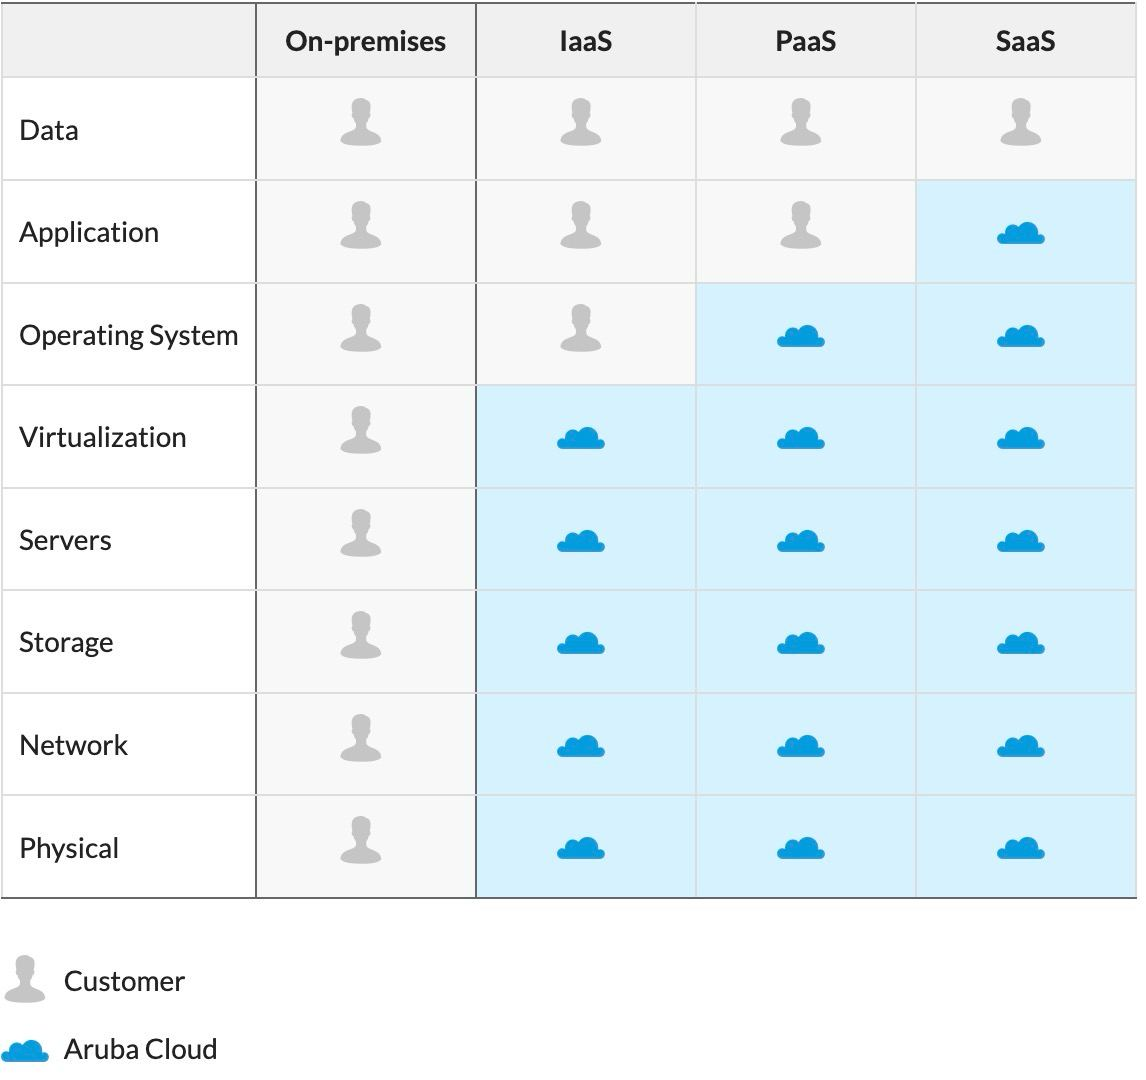
\includegraphics[width=1\textwidth]{aruba-shared-responsibility-model.png}
        \caption{Aruba Shared Responsibility Model}
    \end{figure}

    \newpage
    \subsubsection{AWS Shared Responsibility Model}
    \href{https://aws.amazon.com/it/compliance/shared-responsibility-model/}{AWS Shared Responsibility Model}\footcite{site:aws-shared-responsibility-model} is a model that defines the responsibilities of AWS and the customer for security. AWS is responsible for the security of the cloud, while the customer is responsible for security in the cloud.\\
    It's important to keep in mind that services in services catalogued as \textit{Infrastructure as a Service} (IaaS) the customer is responsible for the security of the operating system and the applications, while in fully managed services the customer is responsible only for the security of the data.\\
    \begin{figure}[htbp]
        \centering
        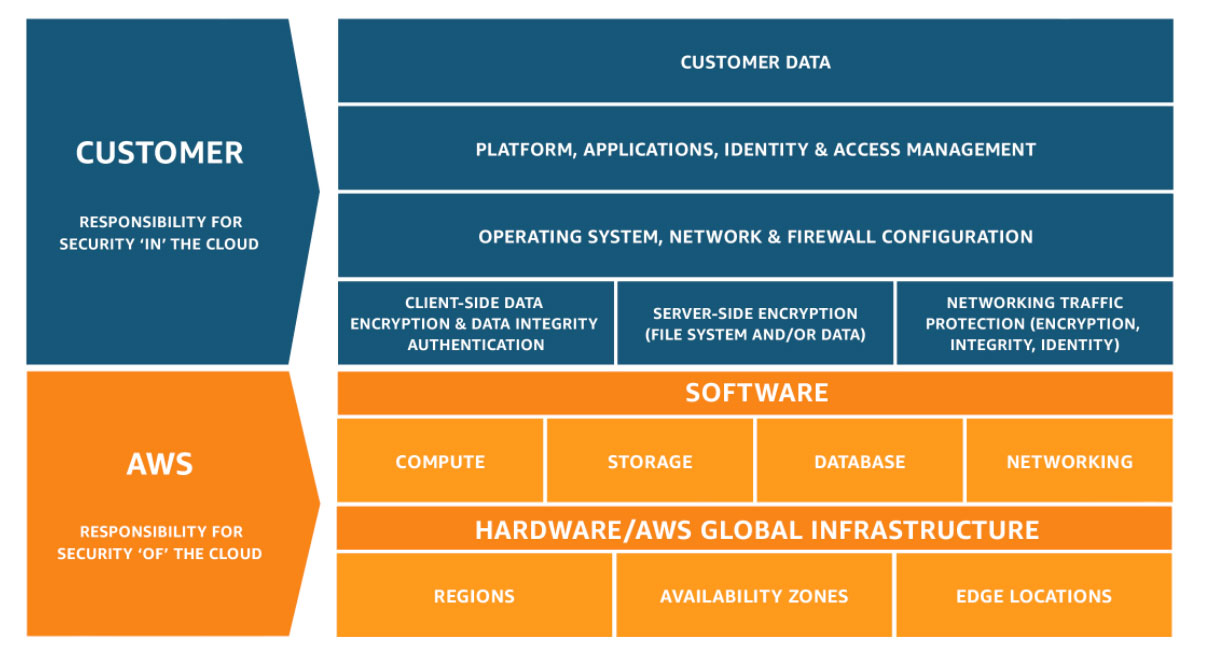
\includegraphics[width=1\textwidth]{aws-shared-responsibility.png}
        \caption{AWS Shared Responsibility Model}
    \end{figure}

    \newpage
    \subsubsection{Azure Shared Responsibility Model}
    \href{https://learn.microsoft.com/en-us/azure/security/fundamentals/shared-responsibility}{Azure Shared Responsibility Model}\footcite{site:azure-shared-responsibility-model} is a model that defines the responsibilities of Microsoft and the customer for security. The responsibility varies depending on wheter the service is \textit{Software as a Service} (SaaS), \textit{Platform as a Service} (PaaS), \textit{Infrastructure as a Service} (IaaS) or on premise. Regardless of the deployment type, the customer always detain data, endpoints account and access management responsibilities.\\
    
    \begin{figure}[htbp]
        \centering
        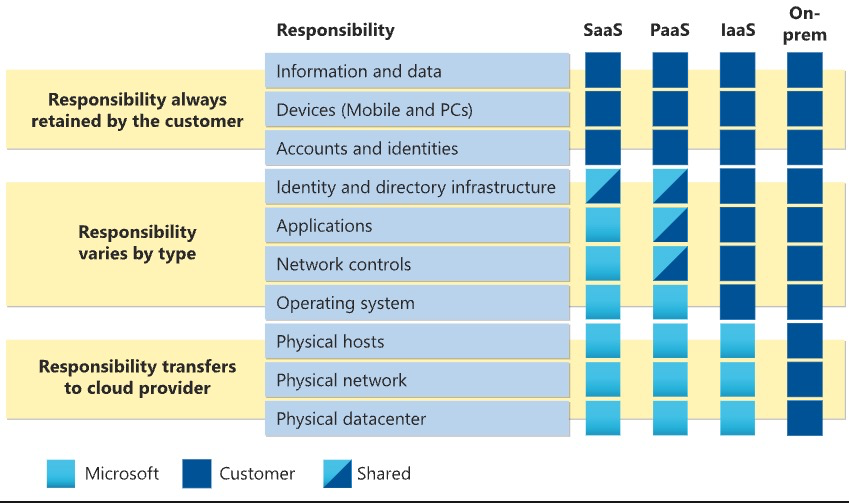
\includegraphics[width=1\textwidth]{azure-shared-responsibility.png}
        \caption{Azure Shared Responsibility Model}
    \end{figure}

\section{Scalability}
The system must be able to scale horizontally by adding more instances of the same service and must be able to scale vertically by increasing the resources of the service. The system must be able to automatically scale based on the load of the system.
Stress tests must be performed to verify the scalability of the system.\\

    \chapter{Methodology}
\label{cap:method}

\intro{In this chapter, we will present the methodology used to develop the proposed solution. The chapter is divided into two sections: architecture, and implementation. The architecture section will present the proposed solution's architecture for the chosen cloud providers, while the implementation section will detail the steps taken to implement the solution.
}\\


\section{Architecture}
\label{sec:architecture}

\begin{figure}[htbp]
    \centering
    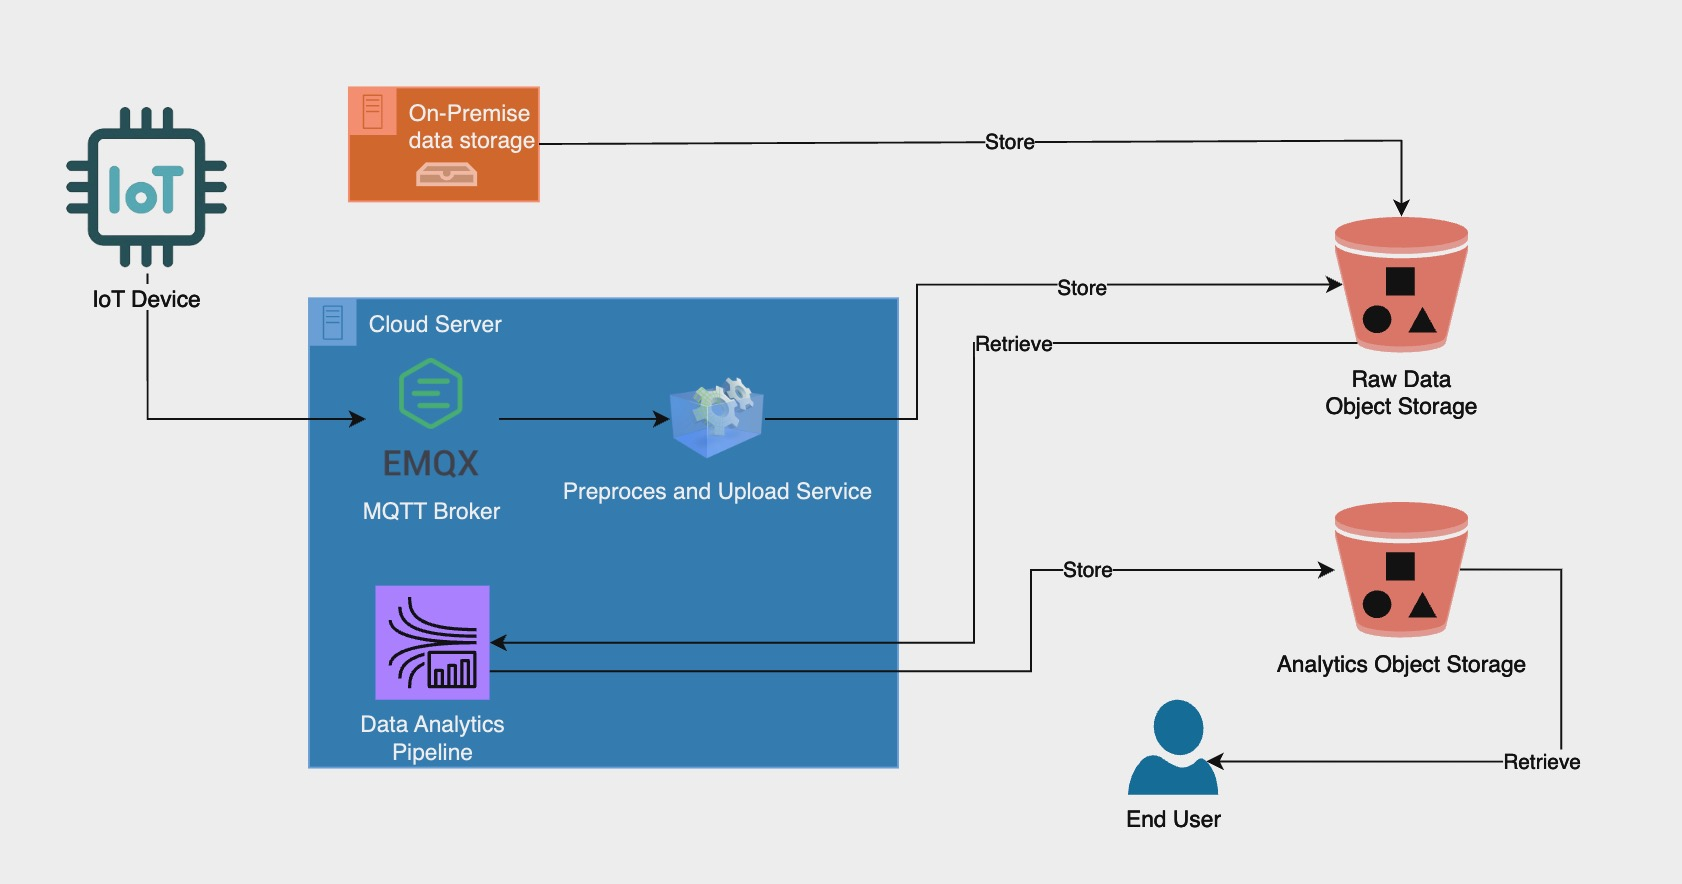
\includegraphics[width=1\textwidth]{architecture.png}
    \caption{Architecture of the proposed solution}
\end{figure}

The proposed solution's architecture consists of a composition of loosely coupled microservices that work together to collect, process, and store data. The architecture is divided into three layers: the data collection layer, the data storage layer and the data analysis layer. Each layer plays a specific role in the overall system, ensuring scalability, flexibility, and resilience.

\subsection{Data Collection Layer}

The data collection layer is responsible for gathering data from IoT devices and archived data. 

\subsection{Data Collection from IoT Devices}

The data collection from IoT devices utilizes the MQTT protocol, a lightweight messaging protocol designed for devices with low bandwidth and high latency. MQTT operates on a publish-subscribe model, where devices publish messages to a broker, which then forwards the messages to subscribers. This protocol is ideal for IoT devices due to its simplicity, ease of implementation, and reliability, with support for different quality of service (QoS) levels to ensure message delivery.

In our scenario, a large number of IoT devices publish data to the cloud. Each device publishes data on a specific topic managed by a cloud-based broker. The data is sent in JSON format, with each message containing a timestamp and a set of key-value pairs representing the data. Once the data is published to the broker, it undergoes preprocessing before being stored in object storage. This preprocessing involves parsing the JSON data, extracting the timestamp and key-value pairs, and converting the data to CSV format. The CSV format was chosen for its simplicity and compatibility with common data processing tools and libraries as well as its reduced verbosity compared to JSON. The preprocessed data is then stored in object storage, making it accessible to the data processing pipeline.


\subsection{Data Collection from Archived Data}
The data collection from archived data is done by uploading files from on-premises to the cloud via a simple script that leverages cloud API. The files, which are already in CSV format, are uploaded to the object storage, where they can be accessed by the data processing pipeline. The files contain historical data that have been collected over time in several different scenarios.

\subsection{Data Storage Layer}

The data storage layer is responsible for storing the raw CSV data and making it accessible to the data processing pipeline. This layer utilizes cloud-based object storage for scalability and durability. The data, always stored in CSV format, is uploaded to the object storage by the data collection layer and accessed by the data analysis layer.
Once the analysis is done, the results are stored in a separate object storage bucket, making them accessible to other services or users.
Object storage provides a reliable and cost-effective solution for storing large amounts of data, with built-in redundancy and scalability features.

\subsection{Data Analysis Layer}

The data analysis layer is responsible for analyzing the collected data and generating insights. This layer consists of several services that retrieve the preprocessed data from the object storage and perform various analytical tasks. The data, initially preprocessed and stored in CSV format, is accessed directly from the object storage by the microservices.

Once the data is retrieved, the microservices perform advanced analytics and machine learning tasks using custom algorithms tailored to specific requirements. These analytical processes transform the raw data into valuable insights, enabling more informed decision-making and a deeper understanding of the underlying patterns and trends in the collected data.
Right after the analysis is done, the results are stored in a separate object storage bucket, making them accessible to other services or users.

\subsection{Cloud Server vs. SaaS Solutions}

The choice of using a cloud server to host both the MQTT broker and the data analytics pipeline provides several advantages over SaaS solutions. While SaaS architectures have been considered, a cloud server offers more flexibility and control over the infrastructure, which is crucial for custom configurations and dependencies required by the data analytics pipeline. It is also more cost-effective for long-term projects, as SaaS solutions typically incur significant monthly fees. A cloud server allows better control over costs, with the trade-off being the need to manage infrastructure and security patches.

Furthermore, this solution is seamlessly implementable with any cloud provider since it doesn't rely on specific services unique to a particular provider. This cloud-agnostic approach allows users to choose the cloud provider that best fits their needs without altering the solution's architecture. Additionally, even though the MQTT broker and the data analytics pipeline are hosted on the same server, they remain independent, respecting the principles of a microservices architecture.

In summary, this architecture provides a robust, scalable, and flexible solution for data collection, processing, and storage, with the added benefit of being cloud-agnostic and cost-effective for long-term deployments.

\section{Test Implementation}

In this section, the base implementation of the proposed solution is presented. The implementation is divided into two main components: the data collection component and the data analysis component. The data collection component is responsible for collecting data from IoT devices and archived data, while the data analysis component is responsible for processing and analyzing the collected data.

\subsection{Data Collection Component}

The data collection component is responsible for collecting data from IoT devices and archived data. This component consists of three main parts: the MQTT broker, the preprocessing pipeline and the data upload script.

\subsubsection{MQTT Broker}
MQTT broker is a lightweight messaging broker that implements the MQTT protocol. The broker is responsible for receiving messages from IoT devices and forwarding them to subscribers. The broker is hosted on a cloud server and is accessible to all IoT devices connected to the network. The broker is configured to use a specific topic for each device, ensuring that messages are delivered to the correct destination. 
The chosen MQTT broker for the test implementation is \href{https://www.emqx.io/}{EMQX}\footcite{site:emqx}, whose pros and cons have been discussed in \ref{emqx}.
Once the broker have been installed and configured in the cloud server, it was tested by connecting some simulated IoT devices and sending messages to the broker. The messages were successfully received by the broker and forwarded to the subscriber, demonstrating the broker's functionality.
The IoT devices used in the test were simulated using the \href{https://mqttx.app/}{MQTTX}\footcite{site:mqttx} client, analyzed in \ref{mqttx}. This MQTT client allows users to simulate IoT devices and publish messages to an MQTT broker. The devices were configured to publish messages to the broker using a specific topic, with each message containing a timestamp and a set of key-value pairs representing the data.

\subsubsection{Preprocessing pipeline}
The preprocessing pipeline is responsible for parsing the JSON data received from the MQTT broker, extracting the timestamp and key-value pairs, and converting the data to CSV format. The pipeline is implemented as a Python script that subscribes to the MQTT broker, receives messages, and preprocesses the data. The script uses the \href{https://pypi.org/project/paho-mqtt/}{Paho MQTT}\footcite{site:paho-mqtt} client library to connect to the broker and receive messages. Once the data is received, it is parsed, and the timestamp and key-value pairs are extracted. The data is then converted to CSV format and stored in object storage. The preprocessing pipeline ensures that the data is in a suitable format for further analysis and processing. The script was tested by connecting it to the MQTT broker and receiving messages from the simulated IoT devices. The messages were successfully parsed, and the data was converted to CSV format, demonstrating the pipeline's functionality.

\subsubsection{Data Upload Script}
The data upload script is responsible for uploading archived data from on-premises to the cloud. The script is implemented as a Python script that uses the cloud provider's API to upload files to object storage. The files contain historical data that have been collected over time in many different scenarios. The script reads the files from a local directory, uploads them to object storage, and makes them accessible to the data processing pipeline. In this scenario the files are already stored in CSV format, making them suitable for direct upload to object storage. The script was tested by uploading several sample files to object storage and verifying that the files were successfully uploaded to the right directory and accessible to the data processing pipeline. 


\subsection{Data Analysis Component}
The data analysis component is responsible for processing and analyzing the collected data. This component can consist of one or more data analytics scripts based on the requirements of the project. Each of the scripts needs to retrieve the correct data from the object storage, perform the required analysis, and store the results in a separate object storage bucket. In the case more than one file needs to be retrieved from storage, the scripts need to manage the data retrieval and processing in parallel to optimize performance and resource usage. The scripts can be implemented in any programming language that supports the required data processing and analysis tasks, such as Python or R. The choice of language depends on the specific requirements of the project and the availability of libraries and tools for data processing and analysis.
This component was tested by implementing a simple data analysis script that retrieves the preprocessed data from object storage, calculates simple statistics, and stores the results in a separate object storage bucket. The script was implemented in Python using various Python libraries such as Pandas and NumPy for data manipulation and analysis. The script was tested by retrieving the preprocessed data from object storage, calculating the statistics, and storing the results in a separate object storage bucket. The results were successfully stored, demonstrating the functionality of the data analysis component.
Once the analytics are uploaded they can be accessed via a web interface or a REST API, depending on the requirements of the project. The results can be visualized using various data visualization tools such as Matplotlib, Plotly, or Tableau, providing insights into the underlying patterns and trends in the collected data.
    \chapter{Results}
\label{cap:results}

\intro{Chapter intro}\\

\section{Tests}



    \chapter{Conclusion}
\label{cap:conclusion}

\intro{In this chapter, the conclusions of the work are presented. The objectives achieved are discussed, as well as the future developments of the project. The author also reflects on what was learned during the development of the project.}\\

\section{Objectives achieved}
The main goal of the project, as described in \ref{sec:objectives-and-requirements} was to develop a scalable cloud-agnostic architecture able to ingest data from multiple sources, process it and store it in a data lake. The architecture was successfully engineered, developed and tested, as described in \ref{cap:method}. The sample architecture has been tested both with \href{https://www.arubacloud.com/}{Aruba Cloud}\footcite{site:aruba-cloud} and \href{https://azure.microsoft.com/it-it/}{Microsoft Azure}\footcite{site:azure} to assess its cloud-agnostic nature.
In chapter \ref{cap:real_implementation} a real-world implementation of the base architecture was presented, showing the flexibility and scalability of the solution. The security constraints were also taken into account and obtained thanks to the shared responsibility model of the cloud providers and the use of encryption at rest and in transit.\\

\section{Future developments}
The future development of the project can be focused both on the base architecture described in chapter \ref{cap:method} and on the real-world implementation described in chapter \ref{cap:real_implementation}.

\subsection{Base architecture}
For the base architecture, the future developments can be focused on the following points:
\begin{itemize}
    \item \textbf{Edge Computing}: the architecture can be extended to support edge computing. A useful feature would be to be able to train machine learning models on the cloud and deploy them on edge devices.
    \item \textbf{Test on other cloud providers}: the architecture can be tested on other cloud providers to assess its cloud-agnostic nature.
\end{itemize}



\subsection{Real World Implementation}

The real-world implementation can benefit a lot more from future developments since it's a real-world use case of the base architecture. The future developments can be focused on the following points:

\subsubsection{Data Ingestion}
\begin{itemize}
    \item \textbf{Mobile Application Integration}:
        \begin{itemize}
            \item Develop a mobile application for data data management and analytics visualization.
            \item Ensure secure data transfer protocols are implemented.
        \end{itemize}
    \item \textbf{Dedicated Hardware}:
        \begin{itemize}
            \item Implement dedicated hardware for direct data upload from suits to the cloud.
        \end{itemize}
\end{itemize}

\subsubsection{Trigger Analytics Pipeline}
\begin{itemize}
    \item \textbf{Event-Driven Services}:
        \begin{itemize}
            \item Implement event-driven services (e.g., cloud functions or serverless architecture) to trigger the analytics pipeline upon data upload.
        \end{itemize}
\end{itemize}

\subsubsection{Data Processing}
\begin{itemize}
    \item \textbf{Advanced Data Preprocessing}:
        \begin{itemize}
            \item Enhance the preprocessing scripts to handle more complex data cleaning and transformation tasks.
        \end{itemize}
    \item \textbf{Enhanced Analytics Algorithms}:
        \begin{itemize}
            \item Develop more sophisticated algorithms for analyzing preprocessed data and extracting detailed insights related to rider performance.
        \end{itemize}
    \item \textbf{Crash Detection Algorithms}:
        \begin{itemize}
            \item Develop specialized algorithms to detect crash events with higher accuracy.
        \end{itemize}
\end{itemize}

\subsubsection{User Access and Notification}
\begin{itemize}
    \item \textbf{User Notification System}:
        \begin{itemize}
            \item Implement push notifications or WebSocket notifications to inform users when their analytics data is ready.
        \end{itemize}
\end{itemize}

\subsubsection{Data Retention and Management}
\begin{itemize}
    \item \textbf{User Download Window}:
        \begin{itemize}
            \item Provide users with a time window to download and save their raw data before it is deleted.
        \end{itemize}
\end{itemize}

\subsubsection{Technical Detail and Tools}
\begin{itemize}
    \item \textbf{Security Enhancements}:
        \begin{itemize}
            \item Enhance security features for API Gateway (e.g., advanced authentication, encryption).
        \end{itemize}
\end{itemize}

\subsubsection{Testing}
\begin{itemize}
    \item \textbf{Automated Unit Testing Framework}:
        \begin{itemize}
            \item Implement an automated unit testing framework to ensure all components are thoroughly tested.
        \end{itemize}
    \item \textbf{Comprehensive Integration Testing}:
        \begin{itemize}
            \item Perform extensive integration testing to validate interactions between all system components.
        \end{itemize}
\end{itemize}

\subsubsection{Additional Enhancements}
\begin{itemize}
    \item \textbf{Performance Optimization}:
        \begin{itemize}
            \item Optimize the performance of the analytics pipeline.
            \item Conduct load testing to ensure the system can handle high data volumes and concurrent users.
        \end{itemize}
    \item \textbf{Scalability Improvements}:
        \begin{itemize}
            \item Enhance the system architecture to support future growth and increased data volume.
            \item Deploy the system on a containerized platform for improved scalability and resource utilization.
        \end{itemize}
\end{itemize}



    %\appendix
   % \chapter{Appendix A}
\section{Java vs Python for API Development}
\label{sec:java-vs-python}

In the realm of API development, Java and Python are two of the most used programming languages, each offering distinct features, benefits, and trade-offs. This section will explore these languages, focusing on their usage in API development with Spring Boot for Java and FastAPI for Python.
A study of the pros and cons of each language and framework will help in determining which one is better suited for API development. Besides the personal experience, the information reported here is based on general industry trends and best practices.

\subsection{Java and Spring Boot}

Java is a statically-typed, object-oriented programming language that has been a staple in enterprise-level applications for decades. Its robustness, extensive libraries, and strong community support make it a reliable choice for large-scale systems.

\textbf{Spring Boot} is a framework designed to simplify the development of Java applications. It is part of the larger Spring Framework ecosystem and is widely used for building production-ready standalone applications with minimal configuration.

\textbf{Pros of Java and Spring Boot:}
\begin{itemize}
    \item \textbf{Performance}: Java's statically-typed nature and JVM optimization result in high performance and efficient memory management, which is crucial for large-scale applications.
    \item \textbf{Scalability}: Java applications, particularly those built with Spring Boot, are known for their scalability. Spring Boot's support for microservices architecture allows for easy scaling and maintenance.
    \item \textbf{Security}: Java offers robust security features, and Spring Boot provides built-in security mechanisms, making it easier to develop secure APIs.
    \item \textbf{Mature Ecosystem}: Java has a mature ecosystem with a variety of libraries, tools, and frameworks. Spring Boot, in particular, integrates seamlessly with other Spring projects and third-party tools.
    \item \textbf{Community Support}: Java's long-standing presence in the industry means it has extensive community support and documentation, which can be invaluable for troubleshooting and development.
\end{itemize}

\textbf{Cons of Java and Spring Boot:}
\begin{itemize}
    \item \textbf{Complexity}: Java's syntax and the Spring Boot framework can be complex and verbose, leading to a steeper learning curve for beginners.
    \item \textbf{Configuration}: Although Spring Boot reduces the configuration overhead compared to traditional Spring applications, it can still be more cumbersome compared to the lightweight configurations in some other languages. A non-experienced developer may find it challenging to set up.
\end{itemize}

\subsection{Python and FastAPI}

Python is a dynamically-typed, interpreted language known for its simplicity and readability. Its versatility and ease of use have made it popular across various domains, including web development, data science, and automation.

\textbf{FastAPI} is a modern, high-performance web framework for building APIs with Python 3.7+ based on standard Python type hints. It is designed to be easy to use and offers automatic interactive API documentation.

\textbf{Pros of Python and FastAPI:}
\begin{itemize}
    \item \textbf{Ease of Use}: Python's simple and readable syntax makes it accessible to beginners and allows for rapid development.
    \item \textbf{Fast Development}: FastAPI leverages Python's dynamic capabilities and type hints to provide features like automatic data validation and interactive API documentation, accelerating development.
    \item \textbf{Flexibility}: Python is highly flexible, and FastAPI's design allows developers to easily integrate with other libraries and tools.
    \item \textbf{Asynchronous Support}: FastAPI natively supports asynchronous programming, making it well-suited for applications requiring high concurrency.
    \item \textbf{Automatic Documentation}: FastAPI automatically generates interactive API documentation using Swagger UI and ReDoc, which is highly beneficial for development and testing.
\end{itemize}

\textbf{Cons of Python and FastAPI:}
\begin{itemize}
    \item \textbf{Performance}: Python, being an interpreted language, is generally slower than compiled languages like Java. This can be a drawback for CPU-intensive tasks.
    \item \textbf{Scalability}: While Python applications can be scaled, it often requires more effort and optimization compared to Java applications. FastAPI, however, improves this aspect with its asynchronous capabilities.
    \item \textbf{Type Safety}: Python's dynamic typing can lead to runtime errors that are not caught at compile time, which can affect the reliability of the code.
\end{itemize}

\subsection{Why Java is a Better Option}

When comparing Java with Spring Boot and Python with FastAPI for API development, Java tends to be a better option for several reasons:

\begin{itemize}
    \item \textbf{Performance and Efficiency}: Java's performance, aided by the JVM, is superior to Python. For API development, where high throughput and low latency are critical, Java's efficiency makes a significant difference.
    \item \textbf{Enterprise-Grade Scalability}: Java's robust ecosystem and the comprehensive features of Spring Boot make it well-suited for large-scale, enterprise-level applications. The scalability and maintainability of Java applications are generally higher, making them ideal for businesses expecting substantial growth.
    \item \textbf{Security}: Java's strong type system and Spring Boot's extensive security features provide a solid foundation for developing secure APIs. This is particularly important for applications handling sensitive data.
    \item \textbf{Community and Ecosystem}: The extensive community support and the mature ecosystem of libraries and frameworks in Java are crucial advantages. Developers have access to a variety of resources, making it easier to find solutions to problems and ensuring long-term project viability.
    \item \textbf{Stability and Reliability}: Java's long history in enterprise environments has proven its stability and reliability. Businesses often prefer Java for critical applications due to its consistent performance and predictable behavior.
\end{itemize}

While Python with FastAPI offers ease of use and rapid development, especially for smaller projects or prototyping, Java with Spring Boot stands out as a more robust, scalable, and secure choice for developing APIs, especially in large-scale and performance-intensive enterprise-level scenarios.







    %\backmatter
    %\printglossary[type=\acronymtype, title=Acronimi e abbreviazioni, toctitle=Acronimi e abbreviazioni]
    %\printglossary[type=main, title=Glossario, toctitle=Glossario]

    \cleardoublepage
\chapter{Bibliografia}

\nocite{*}

% Print book bibliography
\printbibliography[heading=subbibliography,title={Riferimenti bibliografici},type=book]

% Print site bibliography
\printbibliography[heading=subbibliography,title={Siti web consultati},type=online]

\end{document}
